\documentclass[aspectratio=169, 15pt,usenames,dvipsnames]{beamer}
% Source sans

\usepackage[utf8]{inputenc}
\usepackage{fontspec}
\usepackage{sansmathfonts}
\usepackage{xcolor}
\usepackage{fontenc}
\usepackage{unicode-math}
\usepackage{listings}
\usepackage{cprotect}
\usepackage{pgfpages}

\usepackage[makeroom]{cancel}

\usefonttheme{serif}
\usefonttheme{professionalfonts}


\usepackage[sfdefault,scaled=1.1]{FiraSans}
\usepackage{sourcecodepro}
\usepackage{graphicx}

\graphicspath{
    {themes/gd/images/},
    {images/}
}
\usepackage{themes/gd/beamerthemegd}
\usepackage{themes/gd/beamerinnerthemegd}
\usepackage{themes/gd/beamerouterthemegd}
\usepackage{themes/gd/beamercolorthemegd}

\setbeameroption{hide notes} % Only slides
%\setbeameroption{show only notes} % Only notes
% \setbeameroption{show notes on second screen=right}
\setbeamertemplate{note page}{\large\pagecolor{yellow!5}\vfill\insertnote\vfill}

% To give a presentation with the Skim reader (http://skim-app.sourceforge.net) on OSX so
% that you see the notes on your laptop and the slides on the projector, do the following:
% 
% 1. Generate just the presentation (hide notes) and save to slides.pdf
% 2. Generate onlt the notes (show only nodes) and save to notes.pdf
% 3. With Skim open both slides.pdf and notes.pdf
% 4. Click on slides.pdf to bring it to front.
% 5. In Skim, under "View -> Presentation Option -> Synhcronized Noted Document"
%    select notes.pdf.
% 6. Now as you move around in slides.pdf the notes.pdf file will follow you.
% 7. Arrange windows so that notes.pdf is in full screen mode on your laptop
%    and slides.pdf is in presentation mode on the projector.

\graphicspath{
    {themes/gd/images/},
    {images/}
}

\setlength{\parskip}{1em}
\setbeamertemplate{footline}{%
   \raisebox{5pt}{\makebox[\paperwidth]{\hfill\makebox[10pt]{\scriptsize\insertframenumber}}}}

\title{The Streaming Data Platform\\\small as a heavy duty enterprise data marketplace\\\tiny when to use it in your project}

\begin{document}  
\begin{titlePage} 
	\titlepage        
\end{titlePage}
	
\begin{gdsw}
	\frametitle{Hello}
	\centering
\includegraphics[scale=2.3]{denis}
	\\Denis Golovachev		
\end{gdsw} 
\begin{gdsw}
	\centering
\includegraphics[scale=0.3]{gdlogo}
\end{gdsw}
\begin{gdsw}
	\frametitle{SPB}
	\centering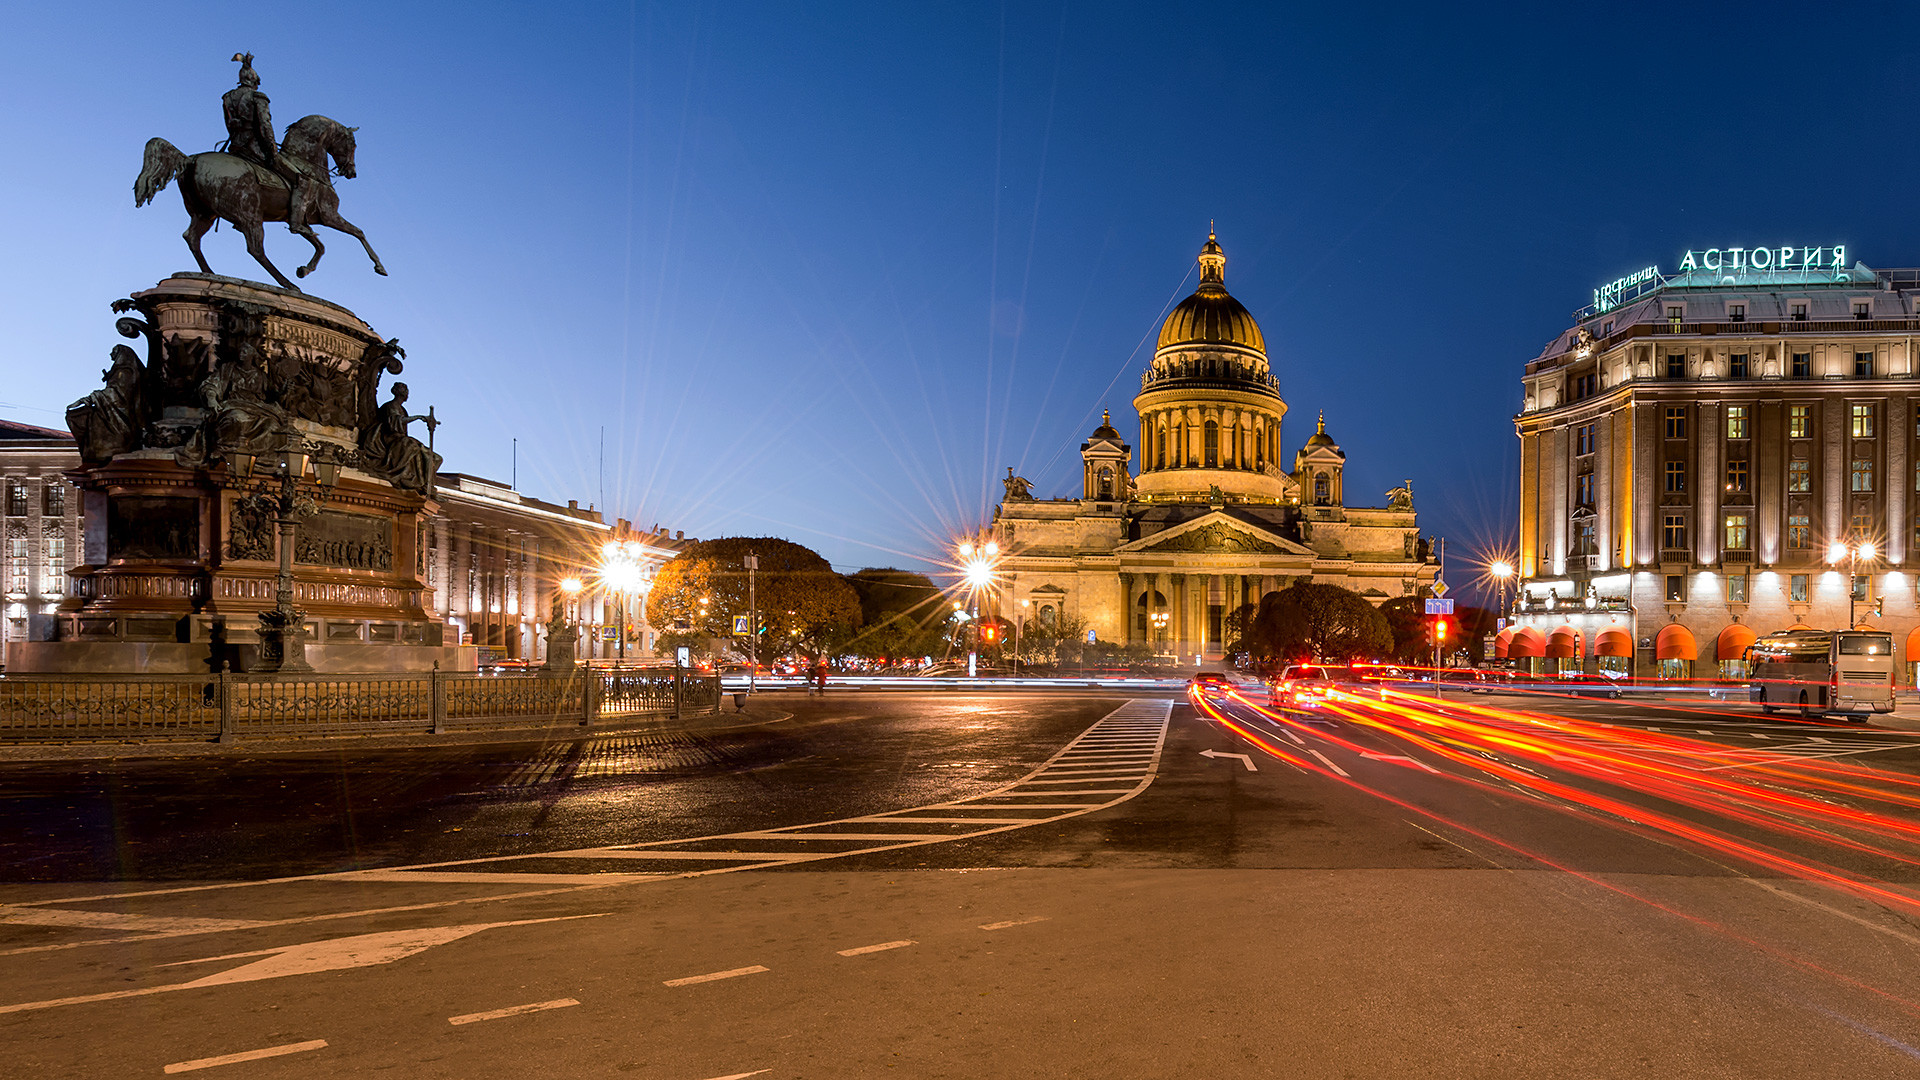
\includegraphics[height=0.7\textheight]{spb}
	\\Saint-Petersburg
\end{gdsw}
\begin{gdsw}
	\centering
\includegraphics[height=0.9\textheight]{bigdata} 
\end{gdsw}
\begin{gdsw}
	\centering
\includegraphics[height=0.7\textheight]{garchitect} 
	\par\LARGE
	Software Architect
\end{gdsw}
\begin{gdsw}
	\frametitle{Data Streaming}
	\centering
\includegraphics[width=0.8\textwidth]{streaming} 
\end{gdsw}
\begin{gdsw}
	\centering\LARGE
	The Streaming Data Platform\\
	as a heavy duty enterprise data marketplace\\
	When to use it in your project.\\
	The case of MMA
\end{gdsw}
\begin{gdsw}
	\centering\LARGE
	{\bf The Streaming Data Platform}\\
	as a heavy duty enterprise data marketplace\\
	{\bf When to use it in your project.}\\
	The case of MMA
	\pause\\
	{\it\small MMA - Multichannel Marketing Automation}
\end{gdsw}
\begin{gdsw}
	\LARGE\centering Small Introduction to
	\centering
\includegraphics[width=0.8\textwidth]{bigdata}
	\par
	Streaming Platforms
	\note{Let's begin\\
		Denis, Architect, engineer, more tech details in this part\\
		Begin with small introduction. Some may have attend, but I'd like to present slightly different view / manner \\
		And as I'm a tech \\
		digits and plots
	}
\end{gdsw}
\begin{gdsw}
	\centering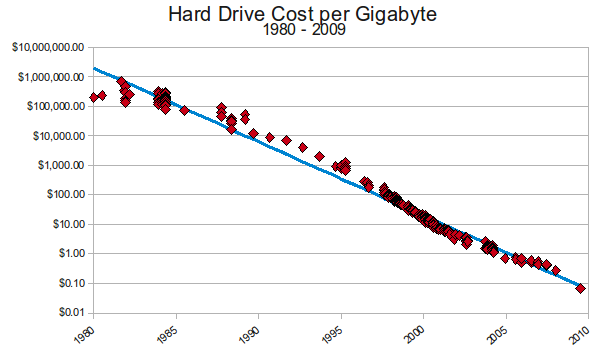
\includegraphics[height=0.6\textheight]{hdd-cost-2} 
	\par	
	For the past 40+ years hard drives prices are constantly dropping
	\note{
		In our electronic devices we usually have HDDs and SSDs as storage\\
		This plot shows how how price changed over the last 40 years\\
		Constantly dropping\\ 
		Twice a year \\
		From around \$500,000 per gigabyte in 1981 to less than \$0.02 per gigabyte today
	}
\end{gdsw}
\begin{gdsw}
	\centering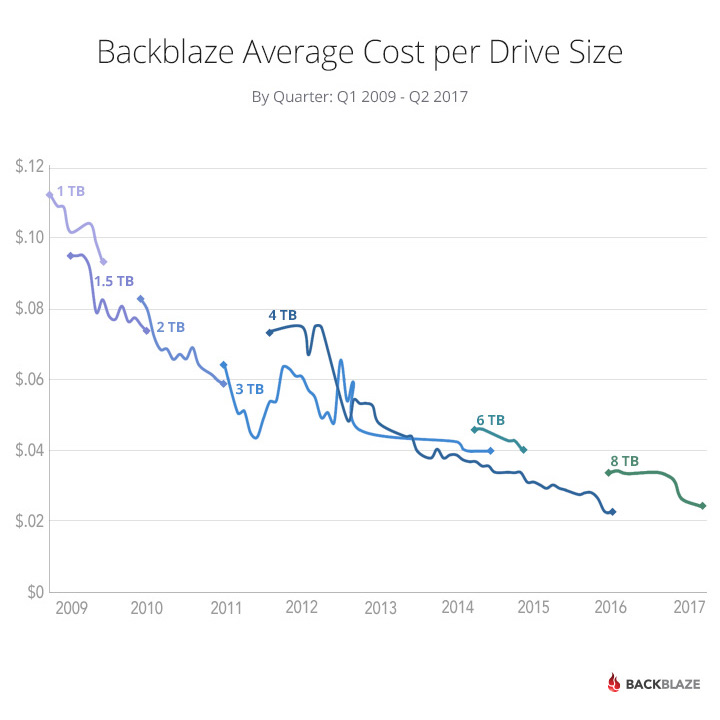
\includegraphics[height=0.6\textheight]{hdd-cost}\\
	\par\normalsize\centering\begin{itemize}
	\item 2010 - countries could store everything. i.e. China
	\item 2015 - big companies could afford to store everything. i.e. Google
	\item 2019 - everyone!
	\end{itemize}
	\note{
		So it became possible somewhere around 2010 for contries to store every data they could collect/intercept/sneak\\
		Sometimes for their survailance programs or even just in case\\
		%Snowden showed that in PRIZM program USA collecting even encrypted data that they could not decrypt just for the furure
		Somewhere in 2015 it become possible for large companies to collect everything
	}
\end{gdsw}
\begin{gdsw}
	\centering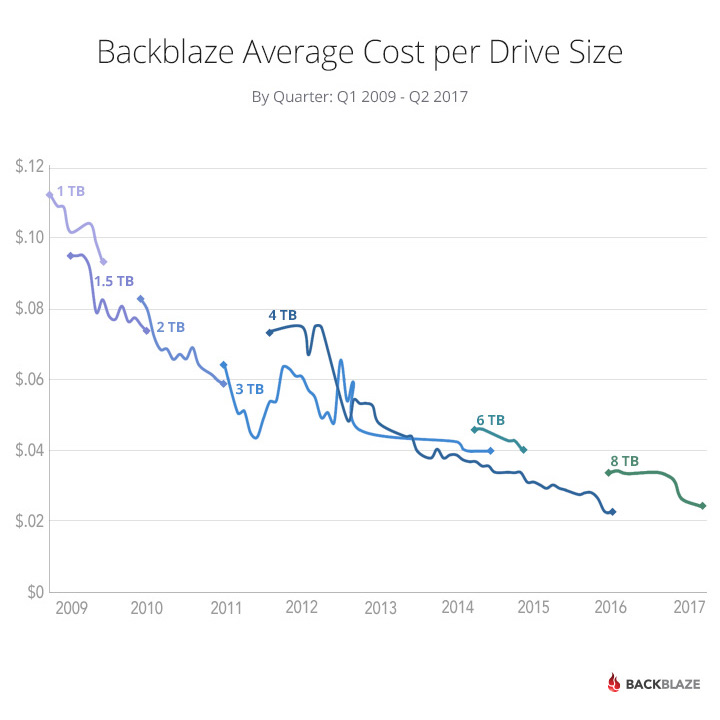
\includegraphics[height=0.6\textheight]{hdd-cost}\\
	\par\Large
	So, the price is low, we store everything. 
	\note{
		And i.e. if we're Facebook it's a question whether we should create a task for our IT guys to clean up outdated data,\\
		And you know that IT time is expensive. So maybe it's better just to buy one more drive for storage.\\
		well this task could take several hours and Facebook IT time is expensive\\
		More than several cents 	
	}	
\end{gdsw}
\begin{gdsw}
	\centering{\fontsize{30}{35pt}\selectfont\bf Information = Money}
	\par\centering\Large
	But could we earn {\bf more} money with all of this information we collecting.\\        
	\note{
		
	}
\end{gdsw}
\begin{gdsw}
	\centering
\includegraphics[height=0.6\textheight]{bigdata}
	\par
	That's what basically we do in our BigData field
	\note{
		And we're good at it
	}
\end{gdsw}
\begin{gdsw}
	\centering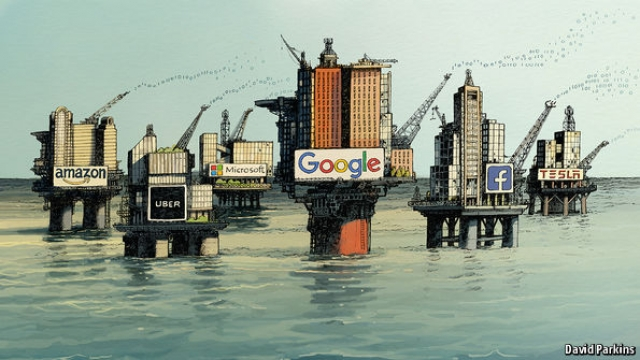
\includegraphics[height=0.6\textheight]{dataoil}
	\par
	The world’s most valuable resource is no longer oil, but data
	\note{
		So nowdays everyone says that\\ the world’s most valuable resource is no longer oil, but data 
	}
\end{gdsw}
\begin{gdsw}
	\centering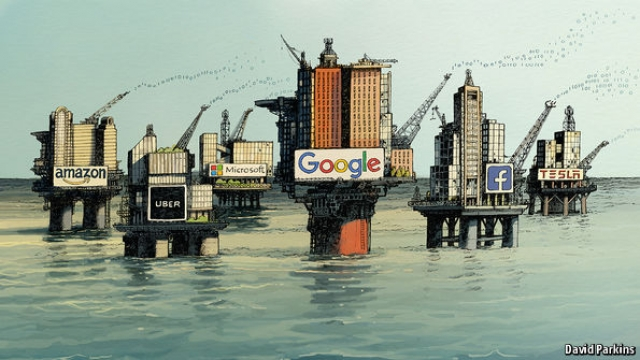
\includegraphics[height=0.3\textheight]{dataoil}
	\par	
	\begin{center}	
		\begin{minipage}{.7\textwidth}			
			\LARGE
			\begin{itemize}
				\item Cheap Storage
				\item Collect Everything
				\item Extract Values
				\item ... Profit
			\end{itemize}
		\end{minipage}
	\end{center}
	\note{
		Time to make profit\\
		But sometimes it's not enough to collect lot of data and extract value from it. Let me explain with example
	}
\end{gdsw}
\begin{gdsw}
	\centering
\includegraphics[width=0.7\textwidth]{knight-capital}
	\par\LARGE
	Do you know this company? 
\end{gdsw}
\begin{gdsw}
	\centering
\includegraphics[width=0.65\textwidth]{knight-capital} 
	\par
	The Knight Capital Group was an American global financial services firm engaging in market making, institutional sales and trading.\\
	With its high-frequency trading algorithms {\bf Knight was the largest trader in U.S}.        
\end{gdsw}
\begin{gdsw}
	\centering
\includegraphics[width=0.6\textwidth]{knight-capital} 
	\par
	\begin{center}\LARGE
		\begin{minipage}{.5\textwidth}
			\begin{itemize}
				\item Lot of Events/Data
				\item Lot of Analytics
			\end{itemize}
		\end{minipage}
	\end{center}
	\note {
		Lot of data - Events, Signals, Markers
	}
\end{gdsw}
\begin{gdsw}
	\centering
\includegraphics[width=0.6\textwidth]{knight-capital} 
	\par
	On August 1st, 2012, Knight Capital deployed a new software update to their production servers.
	They switched it on and immediately they started losing literally \$10 million [£6.4m] a minute.
	\note { 
		Once they deployed a new software update to their production servers\\
		They started losing literally \$10 million a minute\\
		And this went on for 45 minutes. \\At the end of it all they wound up having lost \$440 million 
	}
\end{gdsw}	
\begin{gdsw}
	\centering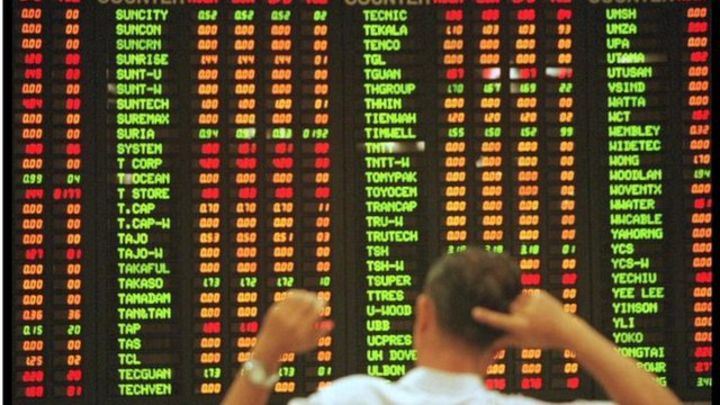
\includegraphics[width=0.65\textwidth]{trading} 
	\par
	{\bf Humans} still {\bf watch the systems}, but {\bf the computers move far too quickly for us to react to everything they do}.\\
	\note{ In a postmortem they said.. \\
		Due to computer glitch the company was making trades it didn't intend to make. \\
		That's guys an example how to lose almost half a billion dollars in a little over half an hour. \\
		It was a fatal day for them
	}
\end{gdsw}
\begin{gdsw}
	\centering{\fontsize{20}{25pt}\selectfont\bf The ability of\\understanding, processing and monitoring huge amount of data fast\\could save you life! }
	\note { 
		conclusion is that sometimes... \\
		Another valuable example is my previous project 
	}
\end{gdsw}
\begin{gdsw}
	\centering
\includegraphics[width=0.7\textwidth]{robbery2} 
	\par
	\LARGE My previous project
	\note{it was connected with fraudsters, we were fighting against them}
\end{gdsw}
\begin{gdsw}
	\centering\includegraphics[width=0.7\textwidth]{fraud-sketch} 
	\par
	\LARGE Fraud Detection System
	\note{
		We had a lot of events. Different kind of them. \\
		Events from our users and with machine learning we were looking for fraudlent behaviour\\
		Anomalies
	}
\end{gdsw}
\begin{gdsw}
	\centering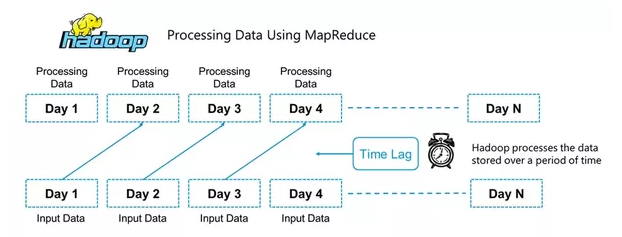
\includegraphics[height=0.6\textheight]{processing-lag} 
	\par
	\begin{center}
		\begin{minipage}{.5\textwidth}		
			\begin{itemize}
				\item Collect - 24hrs
				\item Process - 6hrs
				\item Block Fraudsters - 10 minutes
			\end{itemize}
		\end{minipage}
	\end{center}
	\note {
		Here is First version of Fraud Detection application design\\
		We were collecting 24h of data, processing it for 6 hours and than report some bad guys
	}
\end{gdsw}	
\begin{gdsw}
	\centering\Large We're loosing money!\\
	
\includegraphics[height=0.7\textheight]{itsfine} 
	\par\centering
	\note{
		But once, analytcs department found out that we're loosing money. Quite a lot!\\
		Fraudsters adapted to change their accounts every day, IPs every day, browsers every day. \\
		It's always arms race\\
		And this strategy works for them
	}
	30hr lag \rightarrow {\bf 70 000\$ per day}
\end{gdsw}
\begin{gdsw}
	\centering{\fontsize{30}{35pt}\selectfont\bf What could be improved here?}
	\note{
		Two examples have quite similar flow
	}
\end{gdsw}	
\begin{gdsw}
	\centering{\fontsize{30}{35pt}\selectfont\bf Reaction Time!}
	\note {
		Sometimes it's too late to react
	}
\end{gdsw}
\begin{gdsw}
	\centering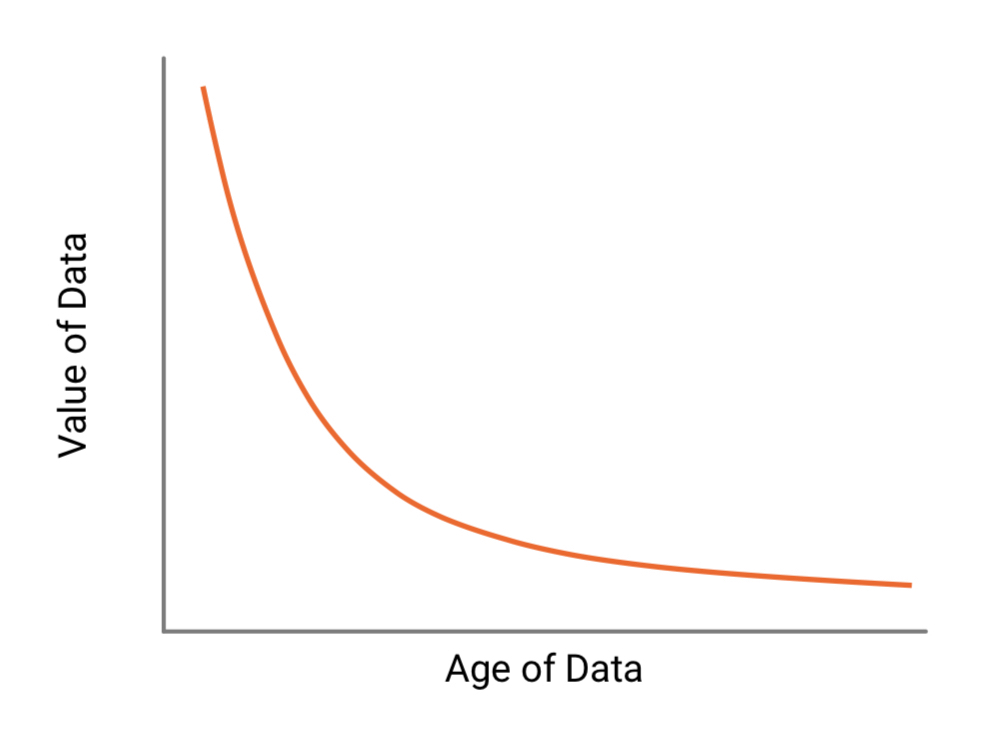
\includegraphics[height=\textheight]{data-aging} 
	\note {
		We could collect lot of data but this data may be useless tomorrow. \\
		Even in 1 hour it may be useless for some sorts of analysis \\
		So we decided to try streaming and 
	}
\end{gdsw}
\begin{gdsw}
	\centering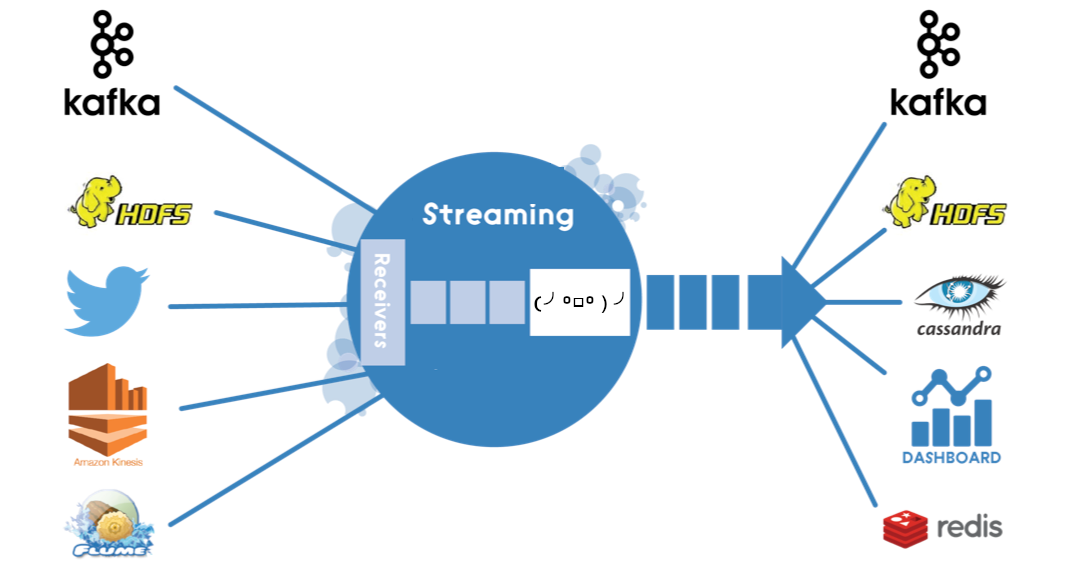
\includegraphics[height=0.7\textheight]{streaming-details} 
	\par\Large
	30 hrs \rightarrow \Rightarrow 10 mins\\
	And Fraudsters were Disappointed
	\note{
		We made it but Knight Capital was not so lucky. \\
		So in general with this kind of streaming solutions we could <next slide>
	}
\end{gdsw}
\begin{gdsw}		
	\begin{columns}
		\begin{column}{0.4\textwidth}
			\centering
\includegraphics[height=0.9\textheight]{gofast} 
		\end{column}
		\begin{column}{0.6\textwidth}
			\large\centering 
			\begin{itemize}
				\item Reduce reaction time
				\item Minimize risk surface
				\item Compete for best offers in market
				\item Give out customers what they need right in time
				\item ...
			\end{itemize}	
		\end{column}
	\end{columns}
	\note {
		Especially for outstanding events\\
		Predict some disasters
	}
\end{gdsw}
\begin{gdsw}
	\centering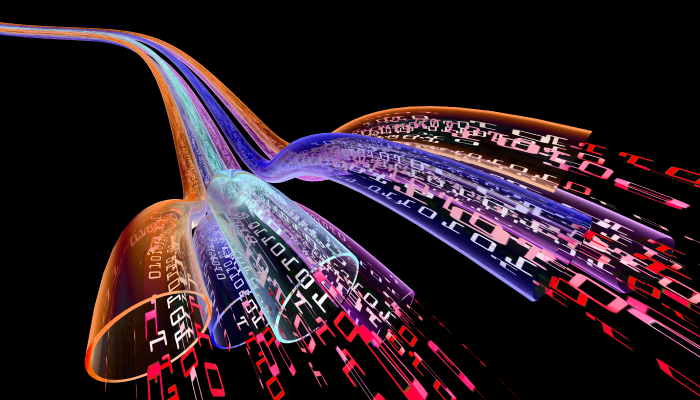
\includegraphics[height=0.6\textheight]{data-streams}\\
	\centering{\fontsize{20}{25pt}\selectfont\bf Streaming Data Platform}
	\note{
		And we're building this kind of platform in Aduno, Streaming Data Platform, SDP project\\
		We're building capability to be fast\\
		Roughly speaking it looks like this
	}
\end{gdsw}
\begin{gdsw}
	\centering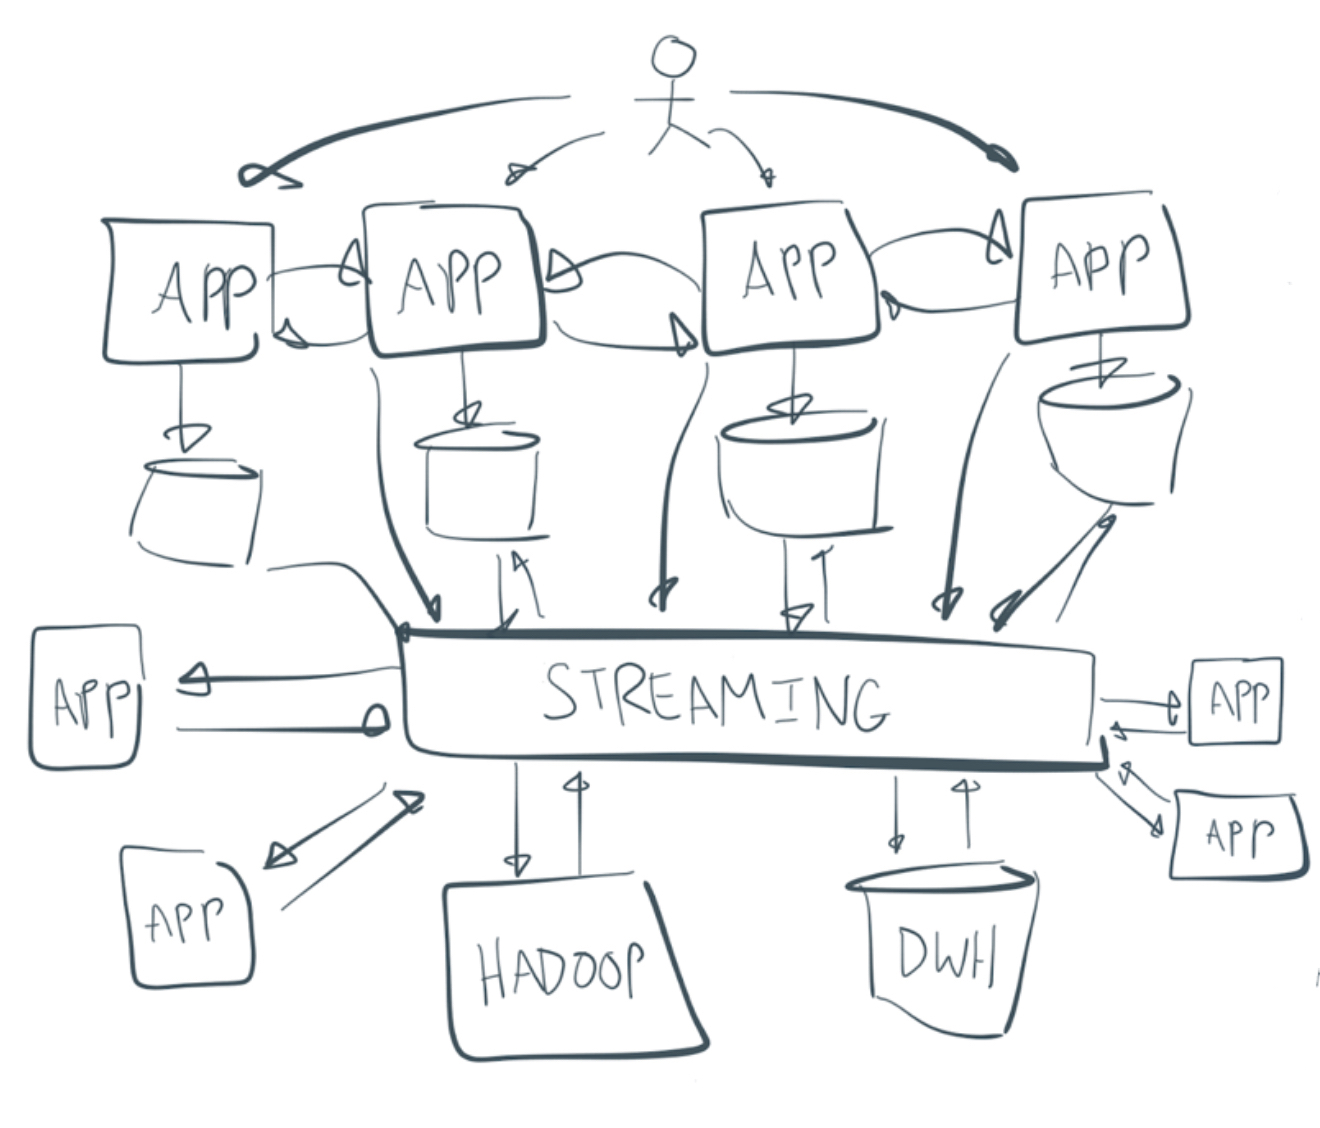
\includegraphics[height=0.6\textheight]{streaming-centering}\\        
	\centering{\fontsize{20}{25pt}\selectfont\bf Streaming Data Platform}
	\note{
		You may say: But we already have something similar.\\ Looks like... wait, Denis \\
		Another magic boxes in the middle
	}
\end{gdsw}
\begin{gdsw}
	\centering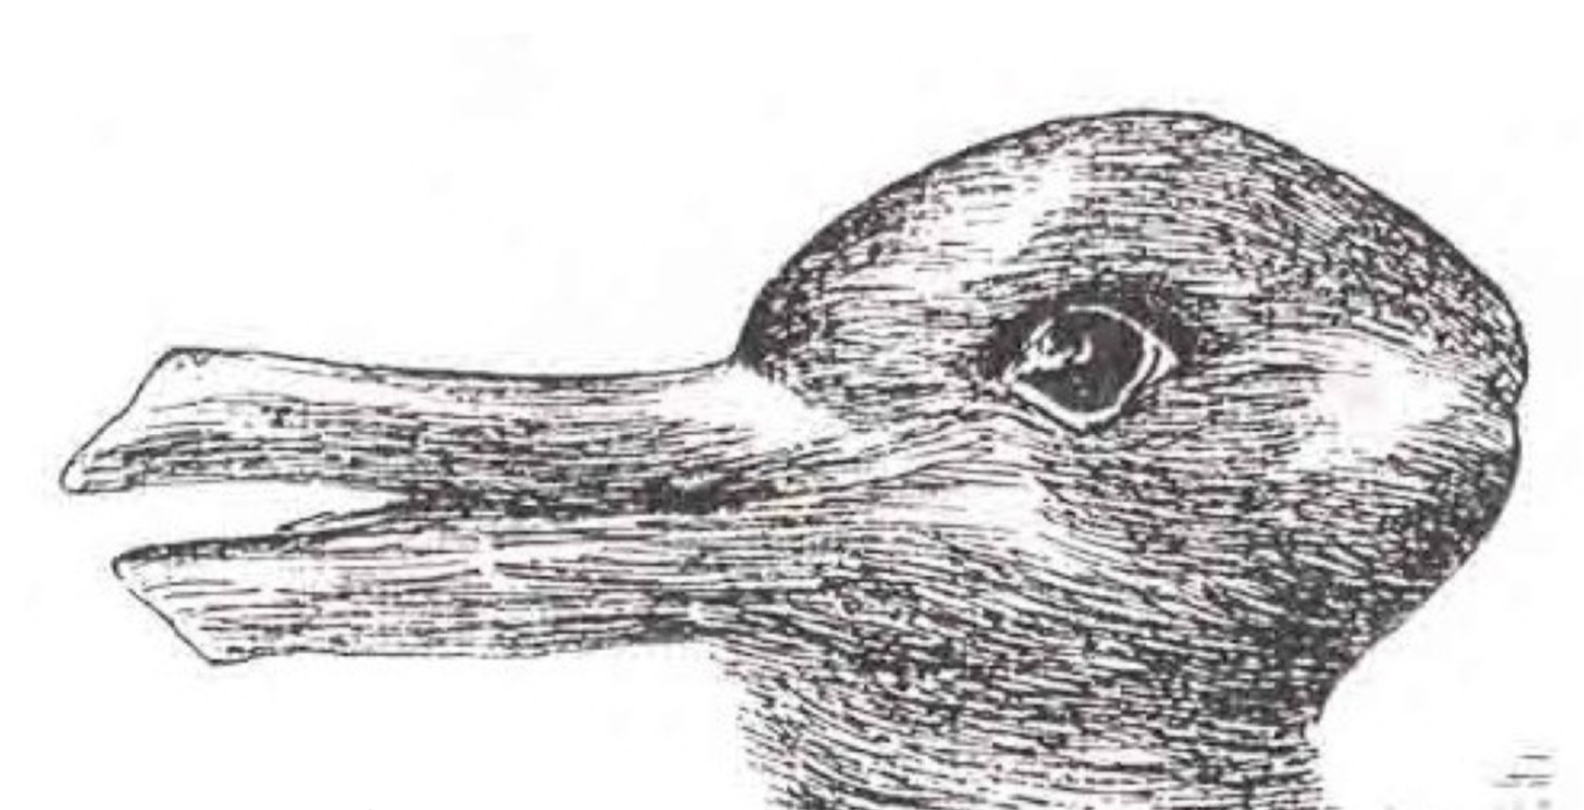
\includegraphics[height=0.5\textheight]{duckrabbit}         
	\par
	\centering{\fontsize{20}{25pt}\selectfont\bf Yet another ESB!?}
	\note{		
		I could explain, but first I should explain some concepts. \\First of all let's take a look at our middleware
	}
\end{gdsw}
\begin{gdsw}
	\centering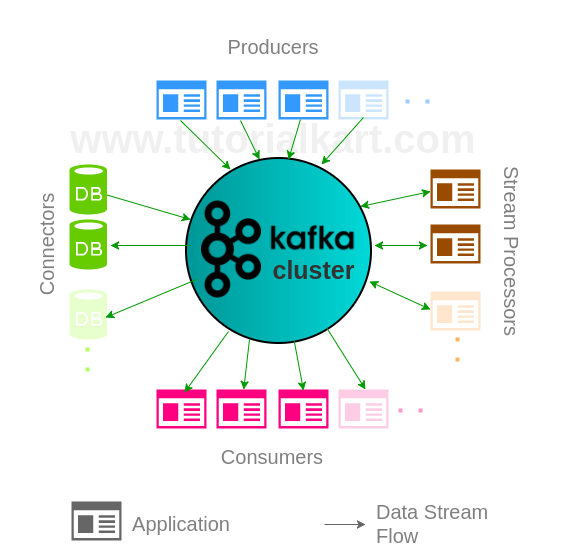
\includegraphics[height=\textheight]{kafka-cluster}  
	\par       
	\centering{\fontsize{20}{25pt}\selectfont\bf Streaming Data Platform}
	\note{
		Kaka - it's database, special case database. Log Storage\\
		Multiple consumers and producers working with immutable log
	}
\end{gdsw}
\begin{gdsw}
	\centering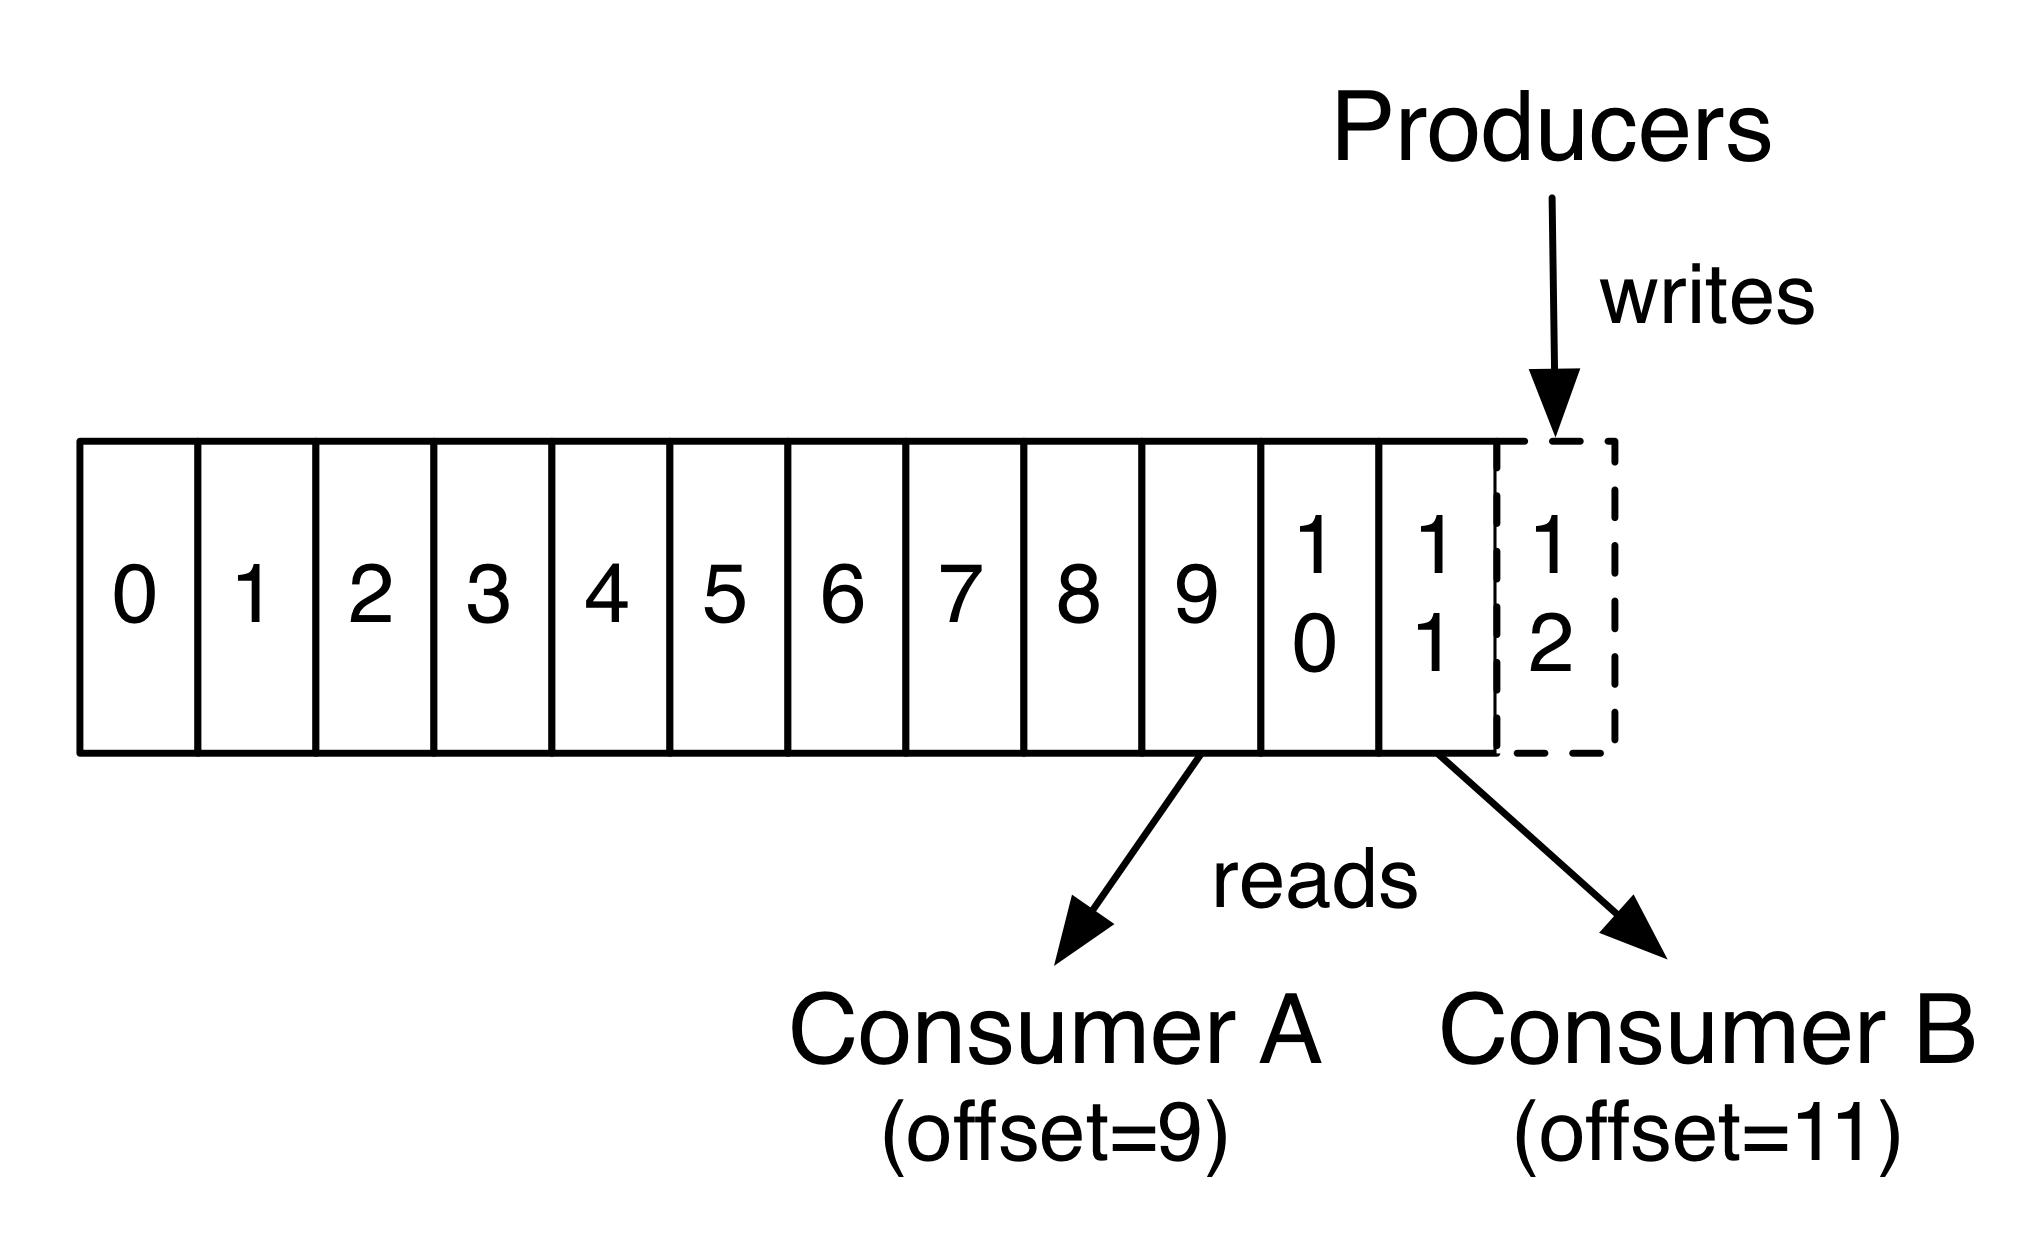
\includegraphics[height=0.7\textheight]{event-log}  
	\par       
	\centering{\fontsize{20}{25pt}\selectfont\bf Immutable event log}
	\note{
		Consumers could shift backward and forward along this immutable log
	}
\end{gdsw}
\begin{gdsw}
	\begin{columns}
		\begin{column}{0.4\textwidth}
			\centering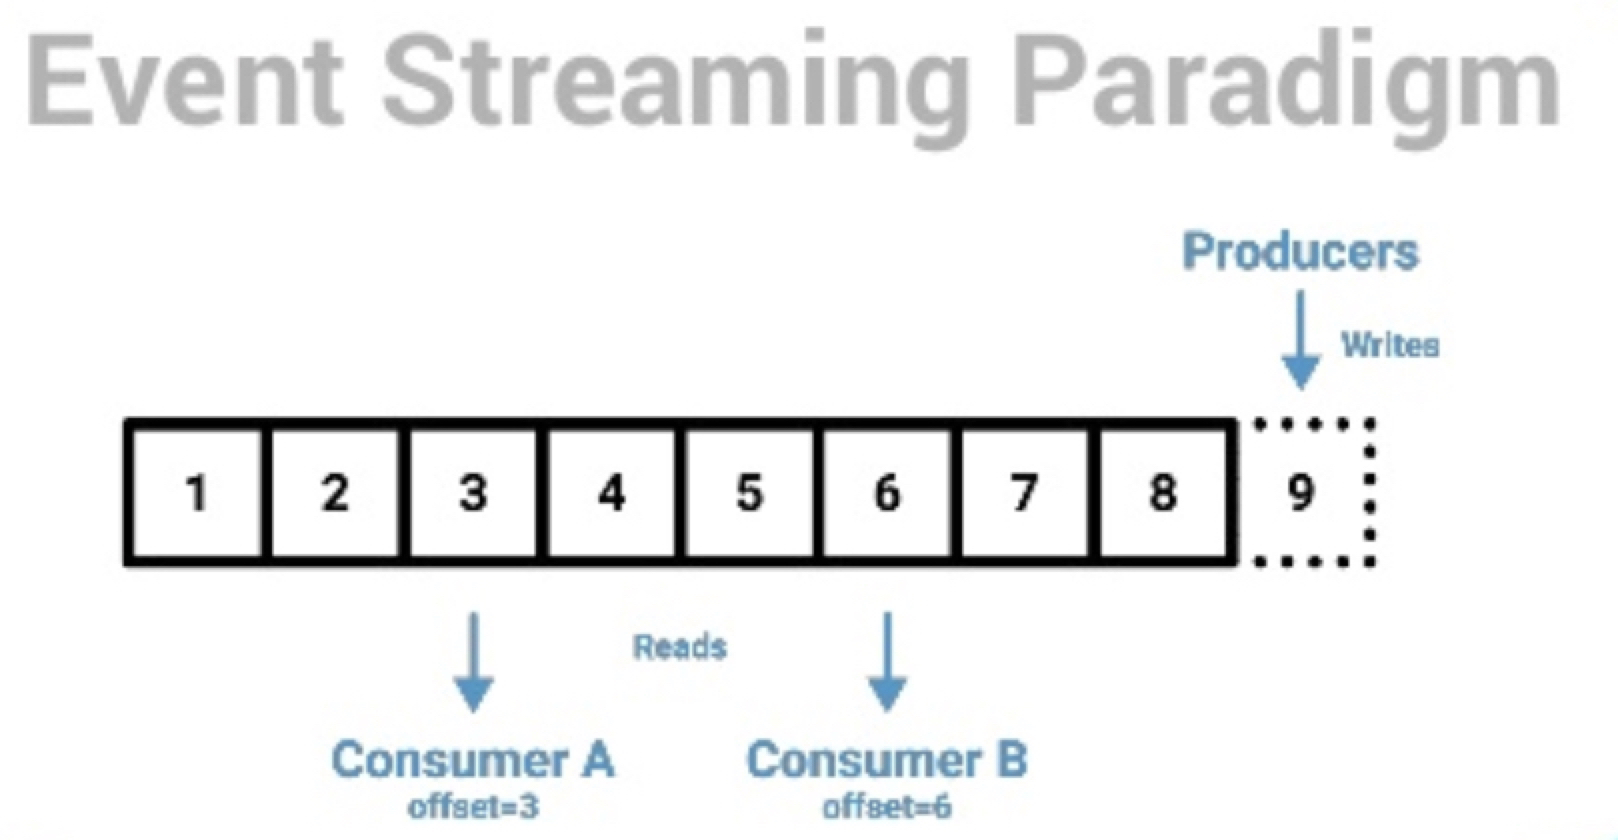
\includegraphics[width=0.9\textwidth]{event-streaming-paradigm} 
		\end{column}
		\begin{column}{0.6\textwidth}
			\large
			\begin{itemize}
				\item Don't route or just processing, it's storage and processing.
				      \pause
				\item Allows downtime for maintenance
				      \pause
				\item Backpressure
				\item Built-in scalability
				      % \item Dumb pipes, smart endpoints
			\end{itemize}	
		\end{column}
	\end{columns}
	\note{
		We could not only consume data in motion, but also use it as database \\	
		Built-in scalability - you don't need another separate broker/cluster for another project\\
		Consumers could read on their own pace\\
		But don't think that SDP and ESBs are enemies, no. they are friends!\\
		They are complementary
	}
\end{gdsw}
\begin{gdsw}
	\begin{columns}
		\begin{column}{0.4\textwidth}
			
\includegraphics[width=0.9\textwidth]{middlewares} 
		\end{column}
		\begin{column}{0.6\textwidth}
			\large
			SDP is scalable, reliable, {\bf but}:
			\begin{itemize}
				\item Integration with legacy
				      \pause
				\item Fast message delivery [Less than a second]
				      \pause
				\item Synchronous Point to Point messaging
				\item Complex Routing
				\item Default protocol is proprietary
			\end{itemize}	
		\end{column}
	\end{columns}	
	\note{
		SDP is not silver bullet\\
		But still there are areas in which we can help. 
	}
\end{gdsw}
\begin{gdsw}
	\centering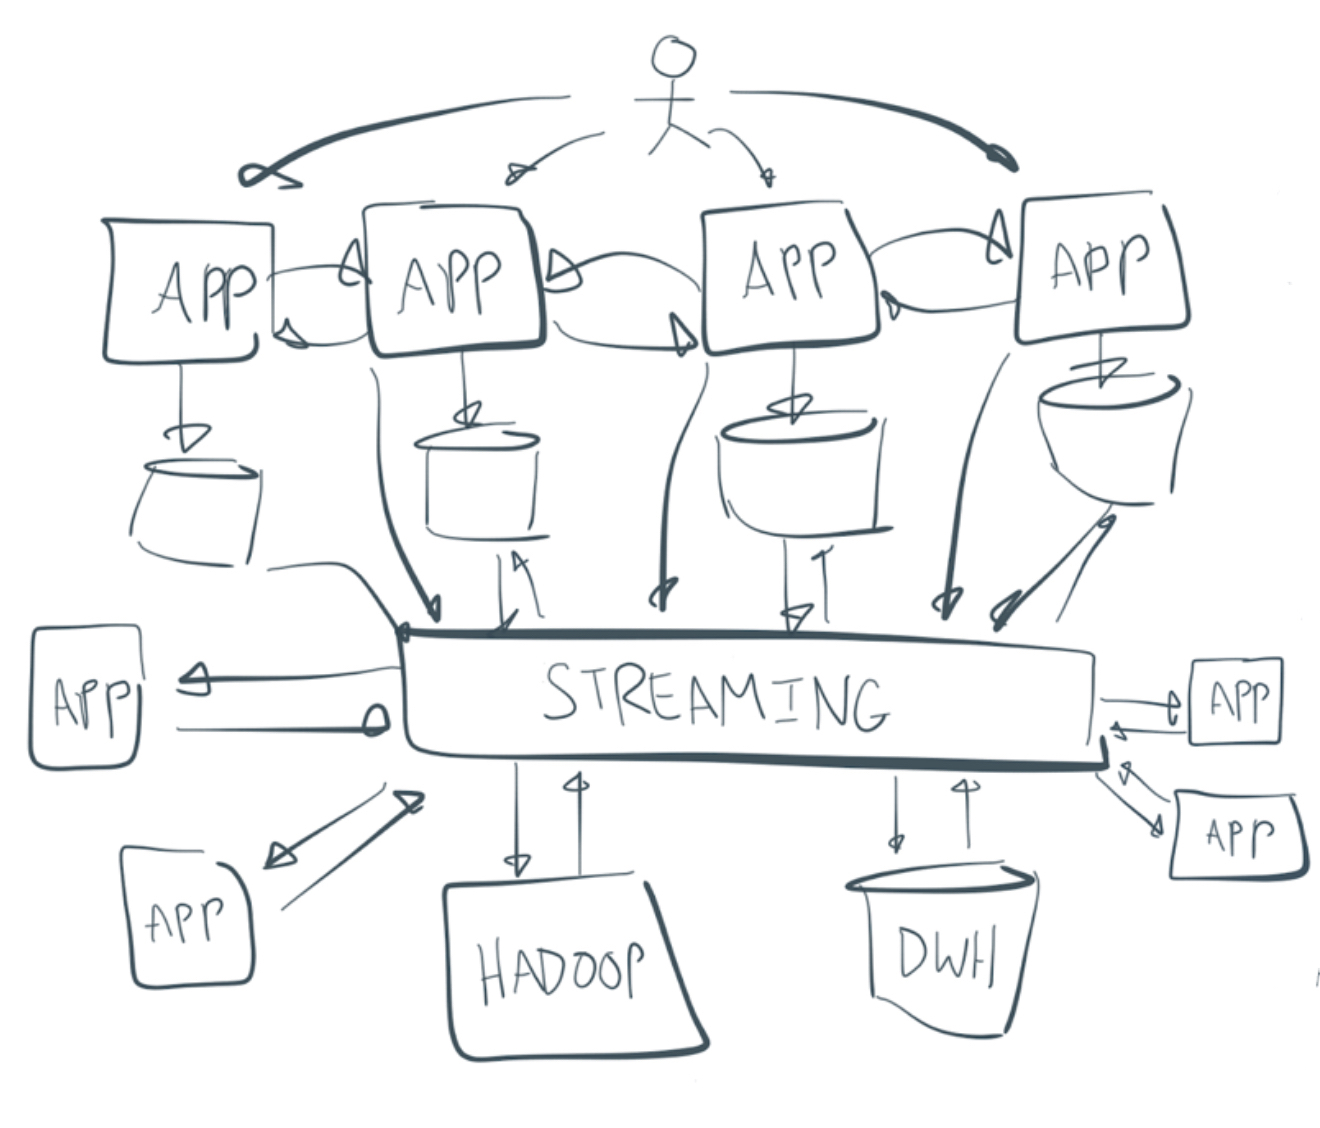
\includegraphics[height=0.3\textheight]{streaming-centering}         
	\begin{center} 
		\begin{itemize}
			\item You have data with short expiration time
			      \pause
			\item You want to reduce data debt
			      \pause
			\item Reaction speed is important for you. Especially for outstanding events
			      \pause
			\item You'd like to build reliable integration between systems. Integration with batteries built-in
			      \pause
			\item You think about how to share your data with other projects
			      \pause
			\item You tired of compliance burden
		\end{itemize}
		\note{
			Data debt - you don't want to find yourself in situation when amount of data you collected is so huge that it becomes hard to analyze. \\
			Complience burden - Security, audit ... we're ready for this.\\
			platform with built-in security\\
			Battaries - reprocessing, zero-dataloss maintenances, backpressure\\
			So if in you project you have this things to solve you should consider SDP\\
			We're always open for your questions and ideas! ty
		}
	\end{center}
\end{gdsw}
\begin{gdsw}
	\centering{\fontsize{20}{25pt}\selectfont\bf Thank you!}
	\par
	References:
	\begin{center}\tiny
		\begin{itemize}
			\item https://en.wikipedia.org/wiki/Knight\_Capital\_Group
			\item https://www.bbc.com/news/magazine-19214294
			\item https://www.backblaze.com/blog/hard-drive-cost-per-gigabyte/
			\item https://www.slideshare.net/KaiWaehner/apache-kafka-vs-integration-middleware-mq-etl-esb
		\end{itemize}
	\end{center}
\end{gdsw}    	
\end{document}
% Not ESB - store and processing data. We could rewind our streams
% The ability of understanding processing and monitoring huge amount of data fast could save you life

% This is how typical ecosystem
% Kafka - immutable
% - Cobol

% 
% we already have something on shelfs and we're going to have more
% you should consider SDP as a solution

% https://en.wikipedia.org/wiki/Knight_Capital_Group
% https://www.bbc.com/news/magazine-19214294
% For hard drive prices, the race to zero is over: nobody won. For the past 35+ years or so, hard drives prices have dropped, from around \$500,000 per gigabyte in 1981 to less than \$0.03 per gigabyte today. 


% https://www.backblaze.com/blog/hard-drive-cost-per-gigabyte/
